%% LaTeX2e template for FEUP's Projeto Integrador
%% 
%% FEUP, JCL, Tue Jan 30 21:57:48 2024
%%
%% PLEASE send improvements to jlopes at fe.up.pt (up till 2028 :-)

%% v2025:
%% - added support for SI Unit rules and style conventions
%% - added acronyms using the corresponding package

\documentclass[11pt,a4paper]{report}

%%------------------------------- preamble ------------------------------------

%% comment next for EN
\usepackage[portuges]{babel}      % language PT 
\usepackage[utf8]{inputenc}       % accents
\usepackage[T1]{fontenc}          % PS fonts
\usepackage{newtxtext,newtxmath}  % do not use CM fonts
\usepackage{amsmath}              % multi-line and other mathematical statements
\usepackage{setspace}             % setting the spacing between lines
\usepackage{graphicx}             % go far beyond what the graphics package
\usepackage[normalem]{ulem}       % various types of underlining
\usepackage{caption}              % rotating captions, sideways captions, etc.
\usepackage{float}                % tables and figures in the multi-column environment 
\usepackage{subcaption}           % for subfigures and the like
\usepackage{longtable}            % tables that continue to the next page
\usepackage{multirow}             % tabular cells spanning multiple rows
\usepackage{booktabs}             % to create professional-quality tables
\usepackage[table]{xcolor}        % driver-independent color extensions
\usepackage{xurl}                 % URL-sensitive line breaks
\usepackage{lipsum}               % loren dummy text
\setlength{\marginparwidth}{2cm}  % todonotes' requirements
\usepackage{todonotes}            % todo's
\usepackage{csquotes}             % context sensitive quotation facilities
\usepackage[backend=biber,authordate]{biblatex-chicago}  % Chicago Manual of Style
\usepackage{pgfgantt}             % Gantt charts
\usepackage[printonlyused]{acronym} % for acronyms
\usepackage{eurosym}              % for the Euro currency symbol
\usepackage{siunitx}              % for SI Unit rules and style conventions
% \sisetup{
%   group-separator = {\,},         % a thin space
%   group-minimum-digits = 4        % enable grouping for numbers ≥ 1000
% }
\DeclareSIUnit{\eurocurrency}{\text{\euro}}  % for the Euro symbol in siunitex

%% document dimensions
\usepackage[a4paper,left=25mm,right=25mm,top=25mm,bottom=25mm,headheight=6mm,footskip=12mm]{geometry}
\setlength{\parindent}{0em}
\setlength{\parskip}{1ex}

%% headers & footers
\usepackage{lastpage}
\usepackage{fancyhdr}
\fancyhf{}                            % clear off all default fancyhdr headers and footers
\rhead{\small{\emph{\projtitle, \projauthor}}}
\rfoot{\small{\thepage\ / \pageref{LastPage}}}
\pagestyle{fancy}                     % apply the fancy header style
\renewcommand{\headrulewidth}{0.4pt}
\renewcommand{\footrulewidth}{0.4pt}

%% colors
\usepackage{color}
\definecolor{engineering}{rgb}{0.549,0.176,0.098}
\definecolor{cloudwhite}{cmyk}{0,0,0,0.025}

%% source-code listings
\usepackage{listings}
\lstset{ %
 language=C,                        % choose the language of the code
 basicstyle=\footnotesize\ttfamily,
 keywordstyle=\bfseries,
 numbers=left,                      % where to put the line-numbers
 numberstyle=\scriptsize\texttt,    % the size of the fonts that are used for the line-numbers
 stepnumber=1,                      % the step between two line-numbers. If it's 1 each line will be numbered
 numbersep=8pt,                     % how far the line-numbers are from the code
 frame=tb,
 float=htb,
 aboveskip=8mm,
 belowskip=4mm,
 backgroundcolor=\color{cloudwhite},
 showspaces=false,                  % show spaces adding particular underscores
 showstringspaces=false,            % underline spaces within strings
 showtabs=false,                    % show tabs within strings adding particular underscores
 tabsize=2,                         % sets default tabsize to 2 spaces
 captionpos=t,                      % sets the caption-position to top
 belowcaptionskip=12pt,             % space between caption and listing
 breaklines=true,                   % sets automatic line breaking
 breakatwhitespace=false,           % sets if automatic breaks should only happen at whitespace
 escapeinside={\%*}{*)},            % if you want to add a comment within your code
 morekeywords={*,var,template,new}  % if you want to add more keywords to the set
}

%% hyperreferences (HREF, URL)
\usepackage{hyperref}
\hypersetup{
    plainpages=false, 
    pdfpagelayout=SinglePage,
    bookmarksopen=false,
    bookmarksnumbered=true,
    breaklinks=true,
    linktocpage,
    colorlinks=true,
    linkcolor=engineering,
    urlcolor=engineering,
    filecolor=engineering,
    citecolor=engineering,
    allcolors=engineering
}

%% path to the figures directory
\graphicspath{{figures/}}

%% bibliography file, must be in preamble
\addbibresource{bibliography.bib}

%% macros to be updated as needed
\newcommand{\school}{Faculdade de Engenharia da Universidade do Porto}
\newcommand{\degree}{Licenciatura em Engenharia Informática e Computação}
\newcommand{\projtitle}{Título do Trabalho}
\newcommand{\subtitle}{Relatório Final do Projeto Integrador}
%\newcommand{\subtitle}{Capstone Project Final Report}
\newcommand{\projauthor}{Nome do Autor}
\newcommand{\supervisor}{Nome do Supervisor}
\newcommand{\tutor}{Prof.\ João Correia Lopes}

%% other macros, if needed
\newcommand{\windspt}{\textsf{WindsPT\/}}
\newcommand{\windscannerpt}{\emph{Windscanner.PT\/}}
\newcommand{\class}[1]{{\normalfont\sffamily #1\/}}
\newcommand{\svg}{\class{SVG}}

%% environments for infos
\newenvironment{info}[1]{\vspace*{6mm}\color{blue}[ \textbf{INFO:} \begin{em} #1}{\vspace*{3mm}\end{em} ]}
\newenvironment{infoopt}[1]{\vspace*{6mm}\color{blue}[ \textbf{INFO (elemento opcional):} \begin{em} #1}{\vspace*{3mm}\end{em} ]}

%%------------------------------- document-------------------------------------

\begin{document}

%% preamble page numbers with roman numerals
\pagenumbering{roman}\setcounter{page}{1}
\pagestyle{plain}

%%------------------------------- cover page ----------------------------------

\begin{titlepage}
\center

\vspace{-15mm}
{\Large \textbf{\textsc{\school}}}\\

\vfill

{\Large \textbf{\projtitle}}\\[8mm]
{\large \textbf{\subtitle}}\\[28mm]

{\Large \textbf{\projauthor}}\\

\vfill


\includegraphics[width=52mm]{uporto-feup.pdf}

\vfill

{\large \textbf{\degree}}\\[8mm]
{\large \textbf{Tutor na U.Porto}: \tutor}\\[2mm]
{\large \textbf{Orientador na empresa}: \supervisor}\\[18mm]

%% fix date if needed
%\renewcommand{\today}{15 de dezembro de 2023}
\today

\end{titlepage}

%%------------------------------- Abstract ------------------------------------

\chapter*{Resumo}

\begin{info}
O resumo tem um caráter essencialmente informativo, devendo ser
escrito de forma concisa (até 200 palavras) de maneira a captar o
interesse de quem o vai ler.

O Resumo substitui a leitura do documento e não contem figuras,
tabelas, citações, etc.\ 
Deve incluir os seguintes tópicos: âmbito, objetivos, os métodos, as
principais descobertas, incluindo resultados, conclusões e
recomendações, se existirem.

Para saber mais sobre como redigir um bom resumo consulte o tutorial
online disponível no website na Biblioteca, ``Guia de Apoio à
Publicação'', secção: 
``\href{https://docs.google.com/document/d/1TDC1behVq8x7fQL4CcPEEh_np5GXviJevQxnQ9gbiJs/edit\#heading=h.s4z9k57ywd9w}
{Estruturar Relatório Técnico}''.
\end{info}

\todo[inline]{Escrever o Resumo, mas só no fim.}

%\vspace{\fill}
%{\Large \textbf{Palavras-chave}:} palavra1, palavra2, palavra3, palavra4
%\vspace*{24mm}

\acresetall %% to reset the acronym usage

%%------------------------------- Acknowledgments -----------------------------

\chapter*{Agradecimentos}

\begin{infoopt}
Habitualmente é mencionada a contribuição de outras pessoas ou
entidades, tanto para a realização do estudo como para a produção do
relatório. 
Podem fazer-se numa página autónoma ou incluir-se na introdução.
\end{infoopt}

%%------------------------------- table of contents ---------------------------

%% redefine tableofcontents text, ONLY for PT
\renewcommand{\contentsname}{Índice}

\tableofcontents

%%------------------------------- list of todos -------------------------------

% list todos; comment in the end (should be empty before delivery :-)
\listoftodos

\begin{infoopt}
Podem ser colocadas anotações durante a preparação do documento, que
são listadas aqui.

Este elemento não aparece no documento final!
\end{infoopt}

%%------------------------------- Acronyms ------------------------------------

\chapter*{Lista de acrónimos}
%\addcontentsline{toc}{chapter}{Lista de acrónimos}

%% sort acronym entries manualy yourself
%% only the acronyms used in the text will be printed

\begin{acronym}[123456] % The longest acronym goes here (for alignment)
  \acro{API}{\textit{Application Programming Interface}}
  \acro{ASCII}{American Standard Code for Information Interchange}
  \acro{GPU}{\textit{Graphics Processing Unit}}
  \acro{FEUP}{Faculdade de Engenharia da Universidade do Porto}
  \acro{IA}{Inteligência Artificial}
  \acro{ML}{\textit{Machine Learning}}
  \acro{PLN}{Processamento de Linguagem Natural}
  \acro{WWW}{World Wide Web}
\end{acronym}

\begin{infoopt}
Justifica-se se estes elementos (acrónimos, unidades, símbolos)
ocorrerem com grande frequência no relatório.

Quando ocorrerem pela primeira vez no texto deve apresentar-se a
respetiva definição.
Por exemplo: Application Programming Interface (API) é uma \ldots 

A lista de itens deve ser manualmante ordenada alfabeticamente.
\end{infoopt}

%%------------------------------- Glossary ------------------------------------

\chapter*{Glossário}
%\addcontentsline{toc}{chapter}{Glossário}

\begin{description}
\item[bash] \hfill \\
  Bash é uma \emph{shell Unix} e uma linguagem de comando escrita 
  em 1989 por Brian Fox para o Projeto GNU como um substituto de 
  software livre para a \emph{Bourne shell}.
\item[firewall] \hfill \\
  Em computação, uma \emph{firewall} é um sistema de segurança de rede 
  que monitoriza e controla o tráfego de entrada e saída da rede 
  com base em regras de segurança predeterminadas.
  Uma \emph{firewall} normalmente estabelece uma barreira entre uma 
  rede confiável e uma rede não confiável, como a Internet.
\item[Glossário] \hfill \\
  Glossário é uma espécie de pequeno dicionário específico para
  palavras e expressões pouco conhecidas presentes num texto, seja
  por serem de natureza técnica, regional ou de outro idioma.
\end{description}

\begin{infoopt}
Justifica-se ter um glossário sempre que seja necessário esclarecer o leitor sobre o significado de terminologia específica usada no texto no relatório.
Recomenda-se a sua localização nos elementos iniciais, embora na
normalização existente haja variantes, podendo também constar nos
elementos finais.

A lista de itens deve ser ordenada alfabeticamente\footnote{%
Para saber mais consulte o tutorial online 
``\href{https://docs.google.com/document/d/1TDC1behVq8x7fQL4CcPEEh_np5GXviJevQxnQ9gbiJs/edit}
{Guia de Apoio à Publicação}''.}.
\end{infoopt}

%%------------------------------- chapter ------------------------------------

\chapter{Introdução}

%% display headers & footers
\pagestyle{fancy}
%% main page numbers with arabic numerals
\pagenumbering{arabic}\setcounter{page}{1}

\begin{info}
Contextualização sucinta do assunto do relatório, fazendo-se
referência ao âmbito e aos objetivos.
Aqui clarifica-se a motivação do trabalho apresentado e explica-se a
abordagem adotada e a sua relação com trabalhos análogos, numa
perspetiva genérica.
Não se deve antecipar detalhes sobre o que é explicado nas secções
posteriores. 
Se for pertinente, pode-se indicar ainda qual o público a que se
destina\footnote{%
Para saber mais consulte o tutorial online 
``\href{https://docs.google.com/document/d/1TDC1behVq8x7fQL4CcPEEh_np5GXviJevQxnQ9gbiJs/edit}
{Guia de Apoio à Publicação}''.}.
\end{info}

Este relatório aborda \ldots\ fornece uma visão geral do contexto, objetivos e abordagem adotada.

\section{Contexto e Motivação}

\begin{info}
   Apresentar o contexto organizacional em que decorreu o projeto/estágio (empresa, instituição, unidade de investigação, laboratório de investigação, etc.). 
   Apresentar o problema abordado e a motivação para o trabalho realizado (qual é o problema abordado e porque é que é importante).
\end{info}

\section{Objetivos e resultados esperados}

\begin{info}
  Indicar os objetivos do trabalho e os resultados esperados.
\end{info}

\section{Estrutura do relatório}
	
\begin{info}
  Descrever brevemente a estrutura do relatório.

  Será expectável que o relatório tenha entre 10 a 25 páginas (em formato A4, coluna única, com um tamanho de letra não excedendo os 12pt no texto de parágrafo), já contando com anexos. 
\end{info}

Para além da introdução, este relatório está organizado em mais 4 capítulos.
No Capítulo~\ref{chap:metodo} \ldots

%%------------------------------- DELETEME ----------------------------------

\newpage  % don't do this
\include{examples}

%%------------------------------- chapter ------------------------------------

\chapter{Metodologia utilizada e principais atividades desenvolvidas}\label{chap:metodo}

Neste capítulo é descrita a metodologia seguida, são enumerados os
principais intervenientes no projeto e é feito o registo das
principais atividades desenvolvidas.

\section{Metodologia utilizada}

\begin{info}
Descrever a metodologia~\parencite{despa2014comparative} seguida (por
exemplo, desenvolvimento iterativo com \emph{sprints} quinzenais e reuniões
semanais de acompanhamento) e os recursos utilizados (por exemplo,
GitHub\footnote{\url{https://github.com/}}, etc.). 
\end{info}

\section{Intervenientes, papéis e responsabilidades}

\begin{info}
Identificar a equipa de projeto, \emph{stakeholders} e outros invernientes com os quais existiu interação; no caso de trabalho em grupo, clarificar os papéis e responsabilidades de cada elemento do grupo.
\end{info}

\section{Atividades desenvolvidas}

\begin{info}
Descrever as atividades realizadas ao londo do tempo (incluindo eventos relevantes, como apresentações, reuniões com clientes, etc.) e respectivos \emph{deliverables}, recorrendo tipicamente a um diagrama de Gantt~\parencite{gantt} (ver Figura~\ref{fig:gantt}) e a uma descrição sumária de cada atividade/\emph{deliverable}.
Pode ser apresentado também através de tabela com progresso semanal.
\end{info}

\begin{figure}
    \begin{ganttchart}[vgrid, hgrid, title height=1,
        x unit=6mm, y unit title=8mm, y unit chart=7mm]{1}{21}

        \gantttitle{Fev.}{4}
        \gantttitle{Mar.}{4}
        \gantttitle{Abr.}{5}
        \gantttitle{Mai.}{4}
        \gantttitle{Jun.}{4} \\

        \gantttitle{0}{1}
        \gantttitle{1}{1}
        \gantttitle{2}{1}
        \gantttitle{3}{1}
        \gantttitle{4}{1}
        \gantttitle{5}{1}
        \gantttitle{6}{1}
        \gantttitle{7}{1}
        \gantttitle{P}{1}
        \gantttitle{8}{1}
        \gantttitle{9}{1}
        \gantttitle{10}{1}
        \gantttitle{11}{1}
        \gantttitle{Q}{1}
        \gantttitle{12}{1}
        \gantttitle{13}{1}
        \gantttitle{14}{1}
        \gantttitle{15}{1}
        \gantttitle{16}{1}
        \gantttitle{17}{1}
        \gantttitle{18}{1} \\

        \ganttbar{\textbf{Reunião kick-off}}{1}{1} \\
        \ganttgroup{Trabalho na empresa}{2}{17} \\
        \ganttbar{\textbf{Reunião intermédia}}{11}{11} \\
        \ganttbar{\textbf{Reunião final}}{18}{18} \\
        \ganttbar{Escrita do Relatório}{18}{20} \\
        \ganttbar{Entregas}{21}{21}
    \end{ganttchart}
    \caption{Diagrama de Gantt.} \label{fig:gantt}
\end{figure}

\chapter{Desenvolvimento da solução}

Neste capítulo é descrito o trabalho desenvolvido para alcançar os
resultados esperados. 
Se for o caso de um protótipo de software, são apresentados os
requisitos, a arquitetura da solução, o desenvolvimento e a validação
do protótipo.

\section{Requisitos}

\begin{info}
Identificar os requisitos funcionais e não funcionais relevantes e respectivas fontes, bem como restrições ao projeto.

Se seguida apresenta-se um exemplo de tabela com \textit{user stories}, que pode ser usada no caso do número de linhas ser grande.
Pode ser necessária mais uma coluna para prioridades.
\end{info}

\subsection*{User stories}

Exemplos de possíveis cenários de utilização são apresentados na Tabela~\ref{tab:userstories}, utilizando \textit{user stories} escritas de acordo com o modelo: 
``\textbf{As a <type of user>, I want <some goal> so that <some reason>}''.

\begin{center}
\begin{longtable}{| c | p{18mm} | p{110mm} |}
\caption{Usage scenario} \label{tab:userstories} \\[-2mm] \hline

\textbf{Identifier} & \textbf{Name} & \textbf{Description} \\ \hline\hline
\endfirsthead

\multicolumn{3}{c}{{\tablename\ \thetable{} -- continued from previous page}} \\[2mm] \hline
\textbf{Identifier} & \textbf{Name} & \textbf{Description} \\ \hline\hline
\endhead

\multicolumn{3}{r}{{Continues on next page\ldots}} \\
\endfoot

\hline
\endlastfoot

US01 & Register (High) & As a \textit{Visitor}, I want to register a new account so that I have access to profile data  \\ \hline

% US02 & Login (High) & As a \textit{Visitor}, I want to login so that % I have access to profile data  \\ \hline
% 
% US03 & Edit profile (High) & As a \textit{Authenticated user}, I want % to edit \ldots\  \\ \hline

\end{longtable}
\end{center}

\section{Arquitetura e tecnologias (ou Conceção e Implementação)}

\begin{info}
Arquitetura e tecnologias utilizadas e respetiva justificação (tendo em conta requisitos e alternativas existentes), diagramas técnicos elaborados (ver Figura~\ref{fig:componentes} retirada de SPARX\footnote{\url{https://sparxsystems.com/resources/tutorials/uml2/component-diagram.html}}), dificuldades técnicas encontradas e sua resolução, etc.
\end{info}

\begin{figure}
\centering
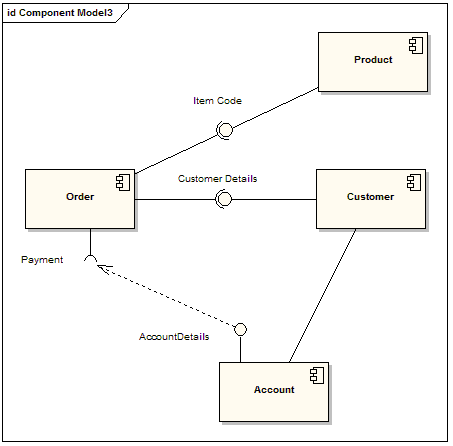
\includegraphics[width=0.72\textwidth]{components}
\caption{Diagrama de Componentes em UML.} \label{fig:componentes}
\end{figure}

\section{Solução desenvolvida}

\begin{info}
Apresentar a solução desenvolvida na ótica do utilizador, com ajuda de \emph{screenshots}.
\end{info}

\section{Validação}

\begin{info}
Descrição da validação da solução desenvolvida, em relação aos requisitos e restrições identificados, e respectivos resultados (por exemplo, resultados de avaliação experimental, testes efetuados, \emph{feedback} de utilizadores ou especialistas, etc.).
\end{info}

\chapter{Conclusões}

Neste capítulo são sumariados os resultados alcançados e as lições
aprendidas.
Finalmente, são apresentadas as limitações do trabalho e são propostas
melhorias e trabalho futuro.

\section{Resultados alcançados}

\begin{info}
Sumariar os resultados alcançados e contribuições (em relação aos  objetivos).

No caso de trabalho em grupo, clarificar as contribuições individuais, em termos qualitativos e quantitativos (percentagem).
\end{info}

\lipsum[10]

\section{Lições aprendidas}

\begin{info}
Refletir sobre as lições aprendidas (tendo em conta os objetivos de aprendizagem).
\end{info}

\lipsum[11]

\section{Trabalho futuro}

\begin{info}
Identificar limitações do trabalho realizado e ideias de melhorias e trabalho futuro.
\end{info}


%%------------------------------- Bibliography --------------------------------

%Aqui deverão constar as referências bibliográficas constantes do texto do relatório e eventual bibliografia relevante consultada durante o projeto.

\renewcommand{\bibname}{Referências bibliográficas}
\printbibliography
\addcontentsline{toc}{chapter}{\refname}  % add it to table of contents

\begin{info}
Na lista final de referências devem constar os trabalhos dos autores
citados de forma abreviada ao longo do texto, obtida automaticamente
com o \class{BibLaTeX}\footnote{\url{https://www.overleaf.com/learn/latex/Bibliography_management_in_LaTeX}}.
A referência bibliográfica é a forma mais desenvolvida de indicar as
fontes de informação em que se baseou. 
\end{info}

%%------------------------------- appendix ------------------------------------

\appendix
\chapter{Um Apêndice}

\begin{infoopt}
Os apêndices e os anexos contêm informação que complementa, apoia e
clarifica o relatório e cuja inclusão no corpo principal do relatório
interferiria com uma boa ordem de apresentação das ideias.

Há uma diferença importante entre apêndices e anexos: ``No apêndice
compilam-se apenas os documentos que são da autoria do autor do
relatório, enquanto no anexo se compilam os documentos de autoria de
outros autores que não o do relatório.''\footnote{%
Para saber mais consulte o tutorial online 
``\href{https://docs.google.com/document/d/1TDC1behVq8x7fQL4CcPEEh_np5GXviJevQxnQ9gbiJs/edit}
{Guia de Apoio à Publicação}''.}
\end{infoopt}

%%------------------------------- the end. ------------------------------------

\end{document}
